% Overleaf entry point. Compiler: pdfLaTeX. Bibliography: BibTeX.
% The official TMLR style files are included and have not been modified.
% Paper figures are generated in English by scripts/results/generate_paper_figures.py.
\documentclass[10pt]{article}
\usepackage{tmlr}
\usepackage[utf8]{inputenc}
\usepackage{amsmath,amssymb}
\usepackage{graphicx}
\usepackage{booktabs,tabularx,array}
\usepackage{microtype}
\usepackage{url}
\usepackage[hidelinks]{hyperref}

\newcommand{\ind}{\mathbb{I}}
\newcommand{\concat}{\mathbin{\|}}
\newcommand{\method}{Advance GraphSAGE}
\newcommand{\metric}[1]{\textnormal{#1}}

\title{Revisiting GNN-Guided Retrieval for Knowledge Graph Question Answering: Architectures, Evidence Subgraphs, and End-to-End Analysis}
\author{Anonymous authors}

\begin{document}
\maketitle

\begin{abstract}
Graph neural retrieval offers a way to connect language-model question answering with explicit relational evidence, but its effectiveness depends on both the retriever and the evidence supplied to the generator. We present an independent implementation and empirical reassessment of this workflow, inspired by GNN-RAG. On a shared, filtered WebQSP evaluation set, we compare six graph neural retrieval architectures, investigate shortest-path and rooted prize-collecting Steiner tree (PCST) evidence construction, and evaluate two language models using three retriever seeds. NBFNet achieves the strongest mean retrieval results, including Hits@10 of 0.921 and gold-answer coverage of 0.877. PCST reduces the evidence from approximately 94 triples to 13--15 triples per question and reduces total language-model token use by approximately 78--80\%. These reductions largely preserve answer-entity coverage but lower final answer quality. Semantic edge costs improve the compactness--quality trade-off over constant costs, while the union of shortest paths produces the best final answers. Conditional analysis shows that the language models omit at least one correct answer in approximately 21--24\% of fully covered shortest-path contexts, rising to approximately 47--48\% with semantic PCST. The results identify the evidence-to-answer transition as a substantial bottleneck and show why entity coverage alone is insufficient for evaluating the usefulness of graph evidence.
\end{abstract}

\section{Introduction}
\label{sec:introduction}

Knowledge graphs organize facts as entities and typed relations, providing an explicit structure for representing and accessing knowledge \citep{hogan2021knowledge}. Answering a natural-language question over such a graph requires more than identifying entities with similar names. The system must connect the entities mentioned in the question to possible answers through relations that express the requested meaning. A correct answer may therefore depend on several intermediate facts, while nearby entities connected through other relations may be irrelevant. This makes the selection of useful evidence a central part of knowledge graph question answering (KGQA).

Retrieval-augmented generation combines external information with a language model's ability to interpret a question and produce an answer \citep{lewis2020rag}. In a graph-based setting, the retrieved object can be a collection of relational facts rather than a passage of prose. Graph neural networks (GNNs) provide a mechanism for propagating information through the graph and ranking candidate answer entities. A subsequent evidence-construction stage can expose the facts connecting those candidates to the question entities, allowing a language model to generate an answer from a smaller, explicit context.

GNN-RAG provides the principal motivation for the workflow studied here: graph neural retrieval identifies candidate answers, shortest paths supply relational evidence, and a language model uses that evidence to answer the question \citep{mavromatis2025gnnrag}. This separation is appealing because the graph retriever and the generator perform different tasks. However, the resulting system also depends on choices within each stage. A generic neighborhood aggregator, a relation-aware model, and a question-conditioned path reasoner need not retrieve the same entities. Likewise, two evidence subgraphs can contain the same answer entities while exposing very different relations around them.

We examine these dependencies through an independent implementation and systematic empirical reassessment of GNN-guided KGQA. The study compares six retrieval architectures, then carries the strongest retriever into an investigation of evidence construction and final generation. In addition to a union of shortest paths, we consider rooted prize-collecting Steiner trees (PCST), motivated by their use for compact graph retrieval in G-Retriever \citep{he2024gretriever}. Candidate ranks determine node prizes, while constant or question-dependent semantic costs determine the price of connecting them.

The investigation addresses three questions. \textbf{RQ1:} How does retrieval architecture affect the ranking and coverage of correct answers? \textbf{RQ2:} How does evidence construction affect compactness and information preservation? \textbf{RQ3:} How does the language model affect final answer quality and the use of available evidence? These questions are evaluated in one pipeline, allowing downstream comparisons to reuse the same upstream predictions.

Our contributions are a modular implementation with separately measurable retrieval, evidence, and generation stages; a comparison of six adapted retrievers under shared data and training controls; an assessment of shortest-path evidence against two rooted PCST cost strategies; and an analysis connecting final answer errors to the availability of correct entities in the supplied context. The empirical scope is the configurations and dataset preparation evaluated in this study. We reassess the underlying methodology and its extensions rather than claim numerical replication of the complete GNN-RAG experimental setting.

The central finding is that strong entity retrieval and high context coverage do not guarantee complete answers. PCST achieves substantial compression with small changes in gold-entity coverage, yet final recall and F1 fall. This motivates evaluating graph evidence through both its retained entities and its usefulness to the downstream generator.

\section{Background and Related Work}
\label{sec:related-work}

\paragraph{Graph neural reasoning.}
GraphSAGE learns node representations through neighborhood aggregation \citep{hamilton2017graphsage}. R-GCN extends graph convolution to multiple relation types using relation-dependent transformations, including parameter sharing through basis decomposition \citep{schlichtkrull2018rgcn}. HGT uses type-dependent projections and attention to model heterogeneous graphs \citep{hu2020hgt}. These methods motivate different ways to represent local graph structure, but their original formulations are not interchangeable KGQA systems. Their input representations, conditioning mechanisms, and answer-scoring heads must be specified when adapting them to retrieval.

Other architectures more directly model a reasoning process. ReaRev derives instructions from the question and revises them using information collected from the graph \citep{mavromatis2022rearev}. NBFNet formulates link prediction through learned path composition and aggregation, inspired by the Bellman--Ford algorithm \citep{zhu2021nbfnet}. Our NBFNet adaptation replaces the query-relation input with a natural-language question representation and scores possible answers relative to the supplied seed entities. The comparison therefore covers shared aggregation, relation-specific computation, adaptive instructions, and path propagation.

\paragraph{Graph retrieval for generation.}
GNN-RAG connects learned candidate retrieval with shortest-path evidence for language-model reasoning \citep{mavromatis2025gnnrag}. G-Retriever studies retrieval-augmented generation over textual graphs and uses a PCST-based formulation to obtain a compact relevant subgraph \citep{he2024gretriever}. These approaches motivate the two evidence families considered here. The classical prize-collecting formulation trades the value of selected nodes against connection costs \citep{goemans1995approximation}; it permits a candidate to be omitted when its prize does not justify its connection.

Our evidence construction differs from a direct reproduction of G-Retriever: prizes come from GNN candidate ranks, the question entities anchor the solution, and the output is a set of original knowledge-graph triples. We compare this construction with shortest-path union while holding the retriever fixed. The contribution is thus an empirical examination of methodological choices within a known retrieval-to-generation pattern, with measurements at intermediate stages as well as at the final answer.

\section{Methodology}
\label{sec:methodology}

\subsection{Problem formulation and common workflow}
\label{sec:workflow}

For each question $q$, let $\mathcal{G}_q=(V_q,E_q)$ be its supplied local graph, where each edge is an original directed triple $(u,r,v)$. Let $S_q\subseteq V_q$ be the valid seed entities supplied with the question and $A_q$ its labeled answer set. A retriever assigns each node a score, from which we construct a ranked candidate list $C_q$. An evidence builder $B$ selects triples $H_q\subseteq E_q$, and a language model $L$ produces a predicted answer set $P_q$:
\begin{equation}
 C_q=\operatorname{Select}(f_\theta(q,\mathcal{G}_q,S_q)),\qquad
 H_q=B(\mathcal{G}_q,S_q,C_q),\qquad
 P_q=L(q,\operatorname{text}(H_q)).
 \label{eq:pipeline}
\end{equation}
The arguments of $f_\theta$ describe the common interface; individual architectures use different subsets of the available question and seed information. Gold labels supervise training and support evaluation, but do not enter candidate selection, evidence optimization, or generation.

Figure~\ref{fig:system-overview} shows the complete workflow. Each stage persists its output, so evidence strategies can reuse a trained retriever and language models can consume the same selected facts. The graph defines the answer-search space: we do not retrieve directly from the complete Freebase database or perform entity linking in this study.

\begin{figure}[t]
 \centering
 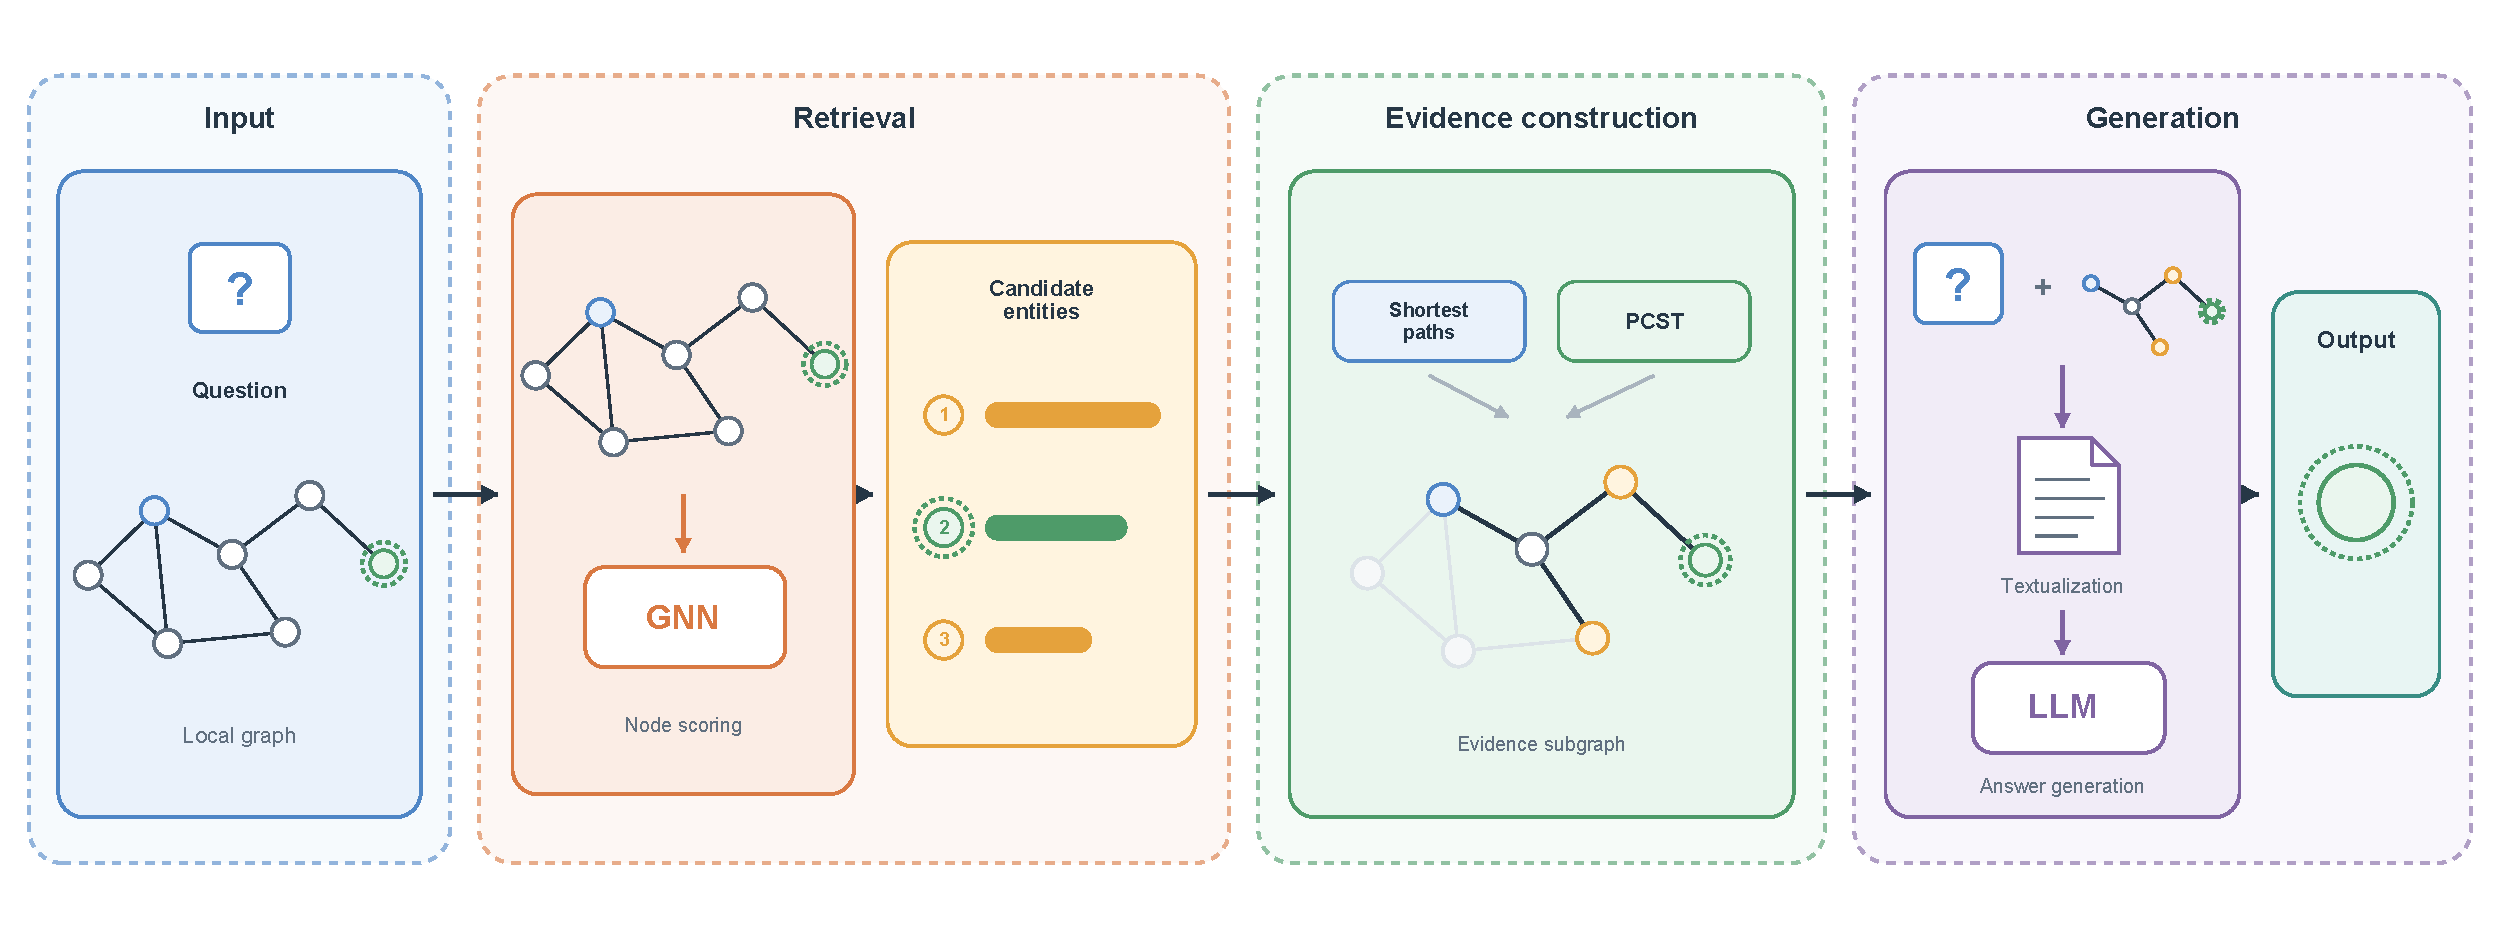
\includegraphics[width=\textwidth]{figures/system_overview.pdf}
 \caption{System overview, from the question and local graph through GNN candidate retrieval, evidence construction, triple textualization, and answer generation. Blue marks a seed, orange marks candidate answers, and the green dotted ring identifies an illustrative gold answer. The gold annotation is explanatory and is not supplied to the system.}
 \label{fig:system-overview}
\end{figure}

\subsection{Retrieval architectures}
\label{sec:architectures}

\paragraph{Shared aggregation and learned question conditioning.}
The GraphSAGE baseline is a weighted adaptation of neighborhood aggregation \citep{hamilton2017graphsage}. Entity embeddings are projected into a hidden space; messages use shared transformations and are weighted by the cosine similarity between question and relation embeddings. A node classifier produces answer logits. Our extension, \method{}, replaces the fixed similarity weight with a learned gate:
\begin{equation}
 \alpha(q,r)=\operatorname{sigmoid}\!\left(\operatorname{MLP}
 [\widetilde{\mathbf q}\concat\widetilde{\mathbf r}\concat
 (\widetilde{\mathbf q}\odot\widetilde{\mathbf r})]\right).
 \label{eq:gate}
\end{equation}
Here $\concat$ denotes concatenation and $\odot$ elementwise multiplication. The extension also adds reverse edges, residual updates, layer normalization, and a classifier conditioned on $[\mathbf h_v\concat\widetilde{\mathbf q}\concat(\mathbf h_v\odot\widetilde{\mathbf q})]$. These changes are evaluated together as one configuration, not as individual ablations.

\paragraph{Relation-aware aggregation.}
R-GCN uses relation-specific transformations with basis decomposition \citep{schlichtkrull2018rgcn}. HGT uses relation-dependent multi-head attention \citep{hu2020hgt}. Because the prepared graphs have one node type, HGT's node-type transformations become shared projections while its relation-dependent operations are retained. In the evaluated implementations, these two models use categorical relation identifiers and node features without direct question conditioning in message passing or their classifier. Consequently, the experiment compares complete retrieval adaptations rather than isolating relation-specific computation alone.

\paragraph{Adaptive instructions and path propagation.}
ReaRev uses a frozen MiniLM encoder for question tokens and relation text, generates multiple instructions, and alternates graph reasoning with instruction revision \citep{mavromatis2022rearev,wang2020minilm}. Its final output is a probability distribution over graph nodes. NBFNet instead initializes seed nodes with a projected question vector and other nodes with zero, retaining this boundary signal during propagation. In layer $\ell$, a relation transformation depends on the question and modulates the source state:
\begin{equation}
 \mathbf w_r^{(\ell)}(\mathbf q)=W_r^{(\ell)}\mathbf q+\mathbf b_r^{(\ell)},
 \qquad
 \mathbf m_{u,r,v}^{(\ell)}=\mathbf h_u^{(\ell)}\odot\mathbf w_r^{(\ell)}(\mathbf q).
 \label{eq:nbfnet}
\end{equation}
This adaptation uses a DistMult-style message operator and principal neighbourhood aggregation (PNA), followed by residual updates and question-conditioned node scoring \citep{yang2015distmult,corso2020pna}. Forward and reverse relations have separate parameters. Architectural settings and training losses are detailed in Appendix~\ref{app:architectures}.

\subsection{Candidate selection}
\label{sec:candidates}

Nodes are ranked by their output probabilities. We retain nodes with probability at least $\tau=0.7$, complete the list with the highest-ranked remaining nodes if fewer than $k=10$ were retained, and cap the result at $K=15$. If the graph has fewer nodes, all available nodes can be retained. This rule applies to every retriever, including ReaRev's normalized distribution. The shared rule controls list size but does not imply that probabilities from different models are equally calibrated.

\subsection{Evidence-subgraph construction}
\label{sec:evidence}

\paragraph{Union of shortest paths.}
For each reachable candidate, we collect all paths of minimum distance from the seed set and take the union of their triples. Structural traversal treats adjacency as undirected, while emitted facts retain their original relation and direction. Multiple equally short paths can therefore contribute additional evidence, and repeated triples are removed. This construction follows the use of shortest-path evidence motivating GNN-RAG \citep{mavromatis2025gnnrag}.

\paragraph{Rooted PCST.}
Let $c_1,\ldots,c_m$ be the valid, reachable candidates in ranked order. Candidate $c_i$ receives prize $\pi(c_i)=m-i+1$, while other nodes have zero candidate prize. We seek a seed-rooted structure with objective
\begin{equation}
 \max_{T}\left[\sum_{v\in V_T}\pi(v)-\sum_{e\in E_T}c(e)\right],
 \qquad
 c_{\mathrm{const}}(e)=\lambda,\quad
 c_{\mathrm{sem}}(e)=\max\{\epsilon,\lambda[1-\cos(\mathbf q,\mathbf r_e)]\}.
 \label{eq:pcst}
\end{equation}
The rooted PCST solver approximates this objective; we do not assume that it returns an exact maximizer. The semantic variant uses question and relation embeddings, with $\epsilon=10^{-6}$ keeping costs positive. A single valid seed is the root. With multiple seeds, a temporary root connects them through zero-cost edges, and sufficiently large additional seed prizes enforce their inclusion. The temporary structure is removed before textualization, so the emitted evidence may have several seed-anchored components.

Both PCST variants operate on original facts represented as undirected structural edges. Parallel relations remain separate possibilities, and artificial reverse edges used by a retriever are not emitted as new facts. Selected edges map back to their original triples. Unlike shortest-path union, PCST can omit a reachable candidate when retaining it is not worthwhile under the prize--cost objective.

\subsection{Answer generation}
\label{sec:generation}

Evidence is serialized as \emph{source $\rightarrow$ relation $\rightarrow$ target}, without free-form paraphrasing. The model receives the original question and these triples, with an instruction to use only the supplied evidence and return a JSON array of complete entity names. An unsupported answer should produce an empty array. The experiments request answers without explanations. After normalization and deduplication, the array is evaluated as a set. Failed calls and invalid generations remain in the evaluation and count as unsuccessful answers; they are not discarded.

\section{Experimental Setup}
\label{sec:setup}

We use the prepared WebQuestionsSP (WebQSP) data associated with Freebase questions \citep{yih2016webqsp}. The available splits contain 2,848 training, 250 validation, and 1,639 test questions. The recorded protocol combines validation and test into 1,889 evaluation questions, excludes 143 whose local graphs lack at least one labeled answer, and evaluates all configurations on the remaining 1,746 questions. Parameters are fitted only on training examples, with the same incomplete-gold filtering policy. This is a conditional evaluation on supplied graphs with full gold availability, not the original unfiltered test-only benchmark protocol.

Retrievers train for 10 epochs with Adam, learning rate $10^{-3}$, zero weight decay, and batches of one graph on an NVIDIA GeForce RTX 5080. Seeds are 42, 1337, and 2026. External embeddings use \texttt{text-embedding-3-small} where required; ReaRev uses its frozen \texttt{all-MiniLM-L6-v2} encoder. Each architecture has one fixed configuration (Appendix~\ref{app:architectures}). NBFNet is carried forward based on the retrieval comparison. Evidence construction evaluates shortest paths and both PCST costs at $\lambda\in\{0.01,0.25,0.5,1\}$. Final generation uses shortest paths and both costs at $\lambda\in\{0.01,1\}$ with the recorded models DeepSeek-V4-Flash and GPT-5.6 Luna. The endpoints retain low- and high-cost conditions without repeating every intermediate value.

We report means and sample standard deviations across the three seed-associated runs. Retrieval uses Hits@1, Hits@10, binary-relevance nDCG@10, and macro gold-answer coverage. Evidence uses triple count, candidate retention, and gold-entity coverage. Final quality uses question-level Hit and Exact Match, together with micro-averaged precision, recall, and F1. Token totals include input and output tokens per run. Context outcomes additionally measure whether all gold answers were returned when all were present in the evidence. Complete definitions and denominators appear in Appendix~\ref{app:metrics}.

\section{Results}
\label{sec:results}

\subsection{Retrieval architecture comparison}
\label{sec:retrieval-results}

Table~\ref{tab:retrieval} reports the six retrievers. NBFNet has the highest mean on every displayed metric: Hits@1 is $0.692\pm0.015$, Hits@10 is $0.921\pm0.005$, and nDCG@10 is $0.796\pm0.007$. Its gold-answer coverage is $0.877\pm0.005$, and all gold answers are retrieved for $0.827\pm0.006$ of evaluated questions. These jointly indicate strong top-rank placement and coverage of multi-answer questions, with little variation across the three runs.

\begin{table}[t]
 \centering
 \caption{Retrieval results on 1,746 questions, mean $\pm$ sample standard deviation across three seeds. RGC is RetrievalGoldCoverage; RFGC is RetrievalFullGoldCoverage. Higher is better for every column. Bold indicates the highest mean, without implying statistical significance.}
 \label{tab:retrieval}
 \begingroup
\small
\setlength{\tabcolsep}{4pt}
\begin{tabular}{@{}lccccc@{}}
\toprule
Architecture & Hits@1 & Hits@10 & nDCG@10 & RGC & RFGC \\
\midrule
GraphSAGE & $0.046\pm0.015$ & $0.252\pm0.034$ & $0.087\pm0.018$ & $0.187\pm0.039$ & $0.129\pm0.031$ \\
\method{} & $0.225\pm0.041$ & $0.801\pm0.019$ & $0.451\pm0.047$ & $0.744\pm0.029$ & $0.644\pm0.036$ \\
R-GCN & $0.121\pm0.076$ & $0.447\pm0.201$ & $0.219\pm0.134$ & $0.393\pm0.200$ & $0.314\pm0.178$ \\
HGT & $0.221\pm0.004$ & $0.671\pm0.016$ & $0.383\pm0.009$ & $0.613\pm0.014$ & $0.518\pm0.017$ \\
ReaRev & $0.588\pm0.103$ & $0.848\pm0.084$ & $0.701\pm0.101$ & $0.771\pm0.088$ & $0.706\pm0.087$ \\
NBFNet & $\mathbf{0.692\pm0.015}$ & $\mathbf{0.921\pm0.005}$ & $\mathbf{0.796\pm0.007}$ & $\mathbf{0.877\pm0.005}$ & $\mathbf{0.827\pm0.006}$ \\
\bottomrule
\end{tabular}
\endgroup

\end{table}

ReaRev is second on the principal ranking measures, with Hits@1 of $0.588\pm0.103$ and nDCG@10 of $0.701\pm0.101$, but its variability is substantially larger. Its mean Hits@10 of 0.848 exceeds \method{}'s 0.801, while the latter is more consistent on this measure. The result favors NBFNet for the subsequent stages because it combines the strongest observed means with stable retrieval; it does not establish that any one of its components causes the advantage.

The difference between GraphSAGE and \method{} is large. Hits@10 rises from 0.252 to 0.801 and gold coverage from 0.187 to 0.744. Learned question--relation weights, reverse edges, residual normalization, and question-conditioned classification together form an effective extension of the baseline. Because these changes were introduced jointly, the experiment cannot assign the improvement to the gate or any other individual component.

R-GCN exhibits the largest standard deviation in Hits@10, $0.201$, around a mean of 0.447. HGT is more stable but remains below \method{} on Hits@10 and gold coverage. Relation-specific transformations and attention therefore do not, by themselves, guarantee better answer retrieval in these adaptations. In particular, the evaluated R-GCN and HGT models lack the direct question conditioning used by the strongest models. The comparison answers RQ1 at the level of the implemented configurations, rather than ranking architecture families independently of their inputs and training choices.

\subsection{Evidence size and information preservation}
\label{sec:evidence-results}

With the same NBFNet predictions, shortest-path union produces $94.47\pm22.58$ triples and $32.12\pm6.60$ distinct nodes per question. Every retrieved candidate is retained under the recorded construction metric. Context gold coverage reaches $0.888\pm0.006$, with full coverage on $0.838\pm0.007$ of questions. Coverage can exceed the retriever's 0.877 because a connecting path can expose a gold entity that was not selected as a candidate.

Figure~\ref{fig:pcst-sensitivity} shows the effect of PCST costs, with complete values in Appendix~\ref{app:evidence-results}. PCST reduces the evidence to 13.50--14.45 triples, approximately 85--86\% fewer than shortest paths. Constant-cost PCST at $\lambda=0.01$ retains all candidates and yields gold coverage of $0.881\pm0.004$, only about 0.7 percentage points below shortest paths. Thus most of the structural compression is achieved by selecting fewer connecting facts, even when no candidates are removed.

\begin{figure}[t]
 \centering
 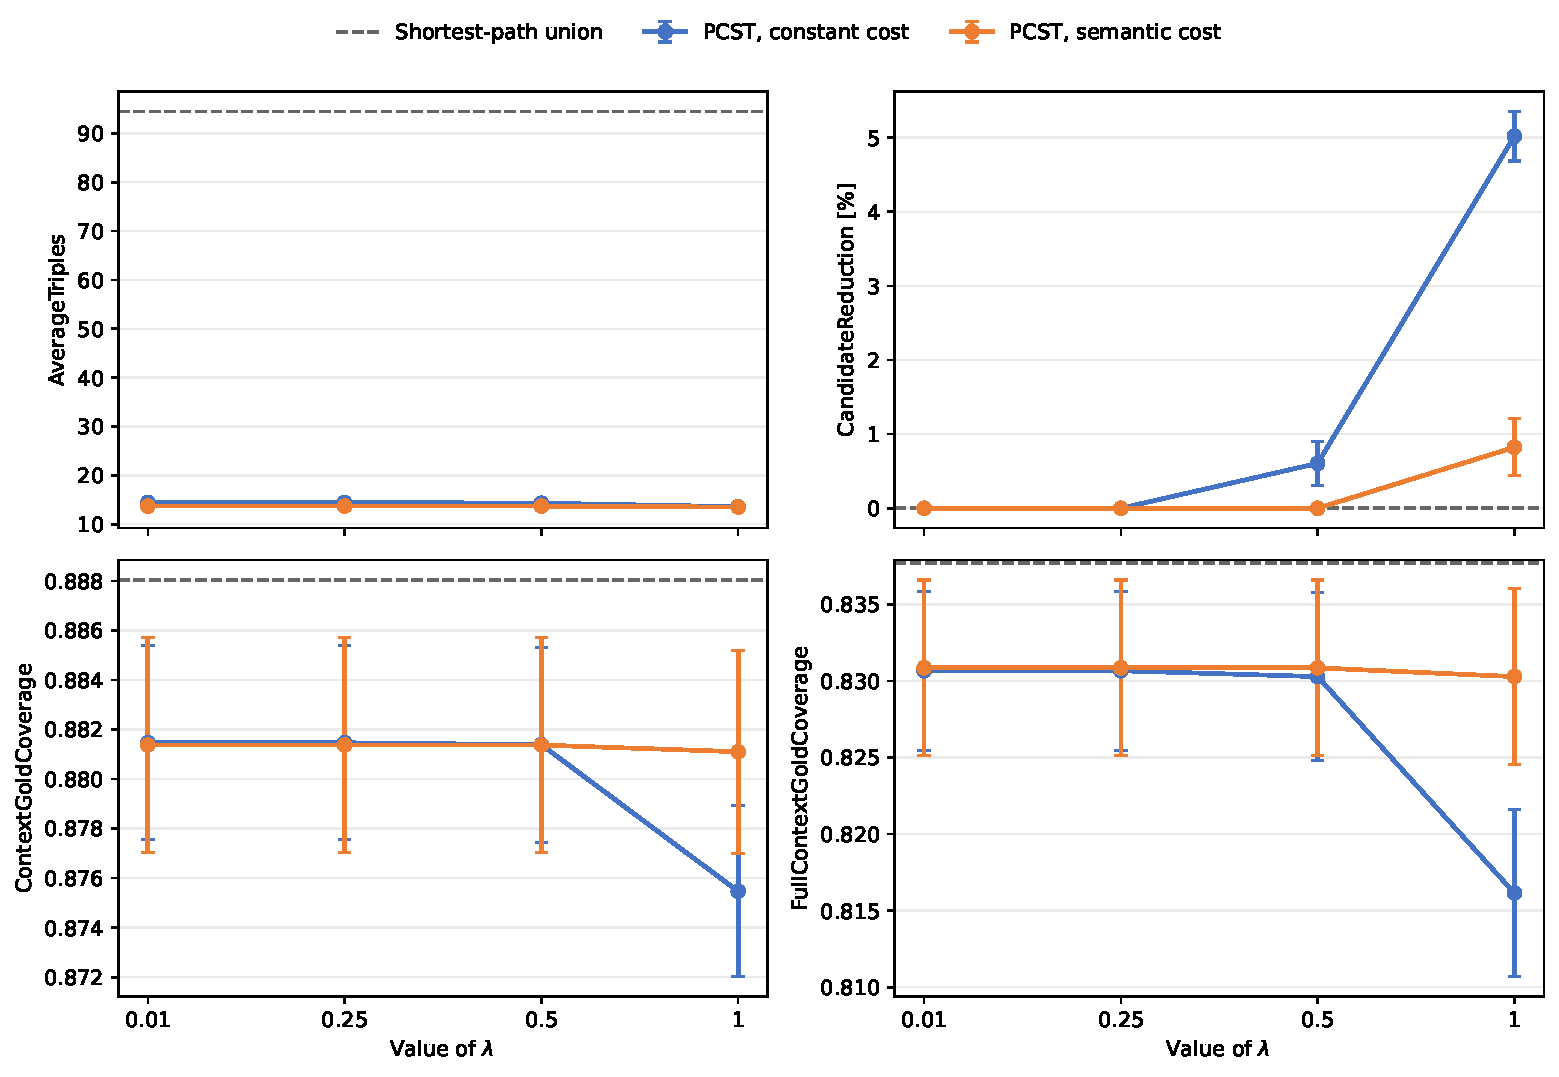
\includegraphics[width=0.86\textwidth]{figures/evidence_pcst_lambda_sensitivity.pdf}
 \caption{Sensitivity of evidence construction to the PCST cost scale. Constant and semantic costs use the same NBFNet retrievers and four values of $\lambda$. Error bars represent standard deviation across three seeds. The accompanying English table in Appendix~\ref{app:evidence-results} reports every configuration and metric.}
 \label{fig:pcst-sensitivity}
\end{figure}

The strongest constant-cost penalty, $\lambda=1$, reduces candidate retention to $0.949\pm0.003$ and removes $5.02\pm0.33\%$ of candidates under the pooled reduction metric. Full context coverage falls to $0.816\pm0.005$. Semantic PCST at the same scale retains $0.991\pm0.004$ of candidates and achieves full coverage of $0.830\pm0.006$ with $13.50\pm0.24$ triples. Semantic costs therefore preserve more candidates at the high-cost endpoint while remaining highly compact.

The aggregate values change little over the lower cost scales. Constant costs at 0.01 and 0.25 yield identical reported aggregates, as do semantic costs at 0.01, 0.25, and 0.5. Aggregate equality does not establish that every individual evidence graph is identical or globally minimal. It does show limited sensitivity of the measured outcomes in that range. For RQ2, the principal result is that major structural compression is possible with small entity-coverage changes; the next stage tests whether that compressed evidence remains equally useful.

\subsection{Final answer quality and token use}
\label{sec:answer-results}

Figure~\ref{fig:quality-tokens} presents the answer-quality and token trade-off. Shortest paths produce the strongest final results for both language models. DeepSeek-V4-Flash reaches Hit $0.802\pm0.005$ and F1 $0.627\pm0.008$; GPT-5.6 Luna reaches Hit $0.804\pm0.015$ and F1 $0.613\pm0.006$. Although their Hit means are close, DeepSeek has higher precision, recall, F1, and Exact Match in this condition. A question-level hit therefore hides differences in how completely and selectively the models return multi-answer sets.

\begin{figure}[t]
 \centering
 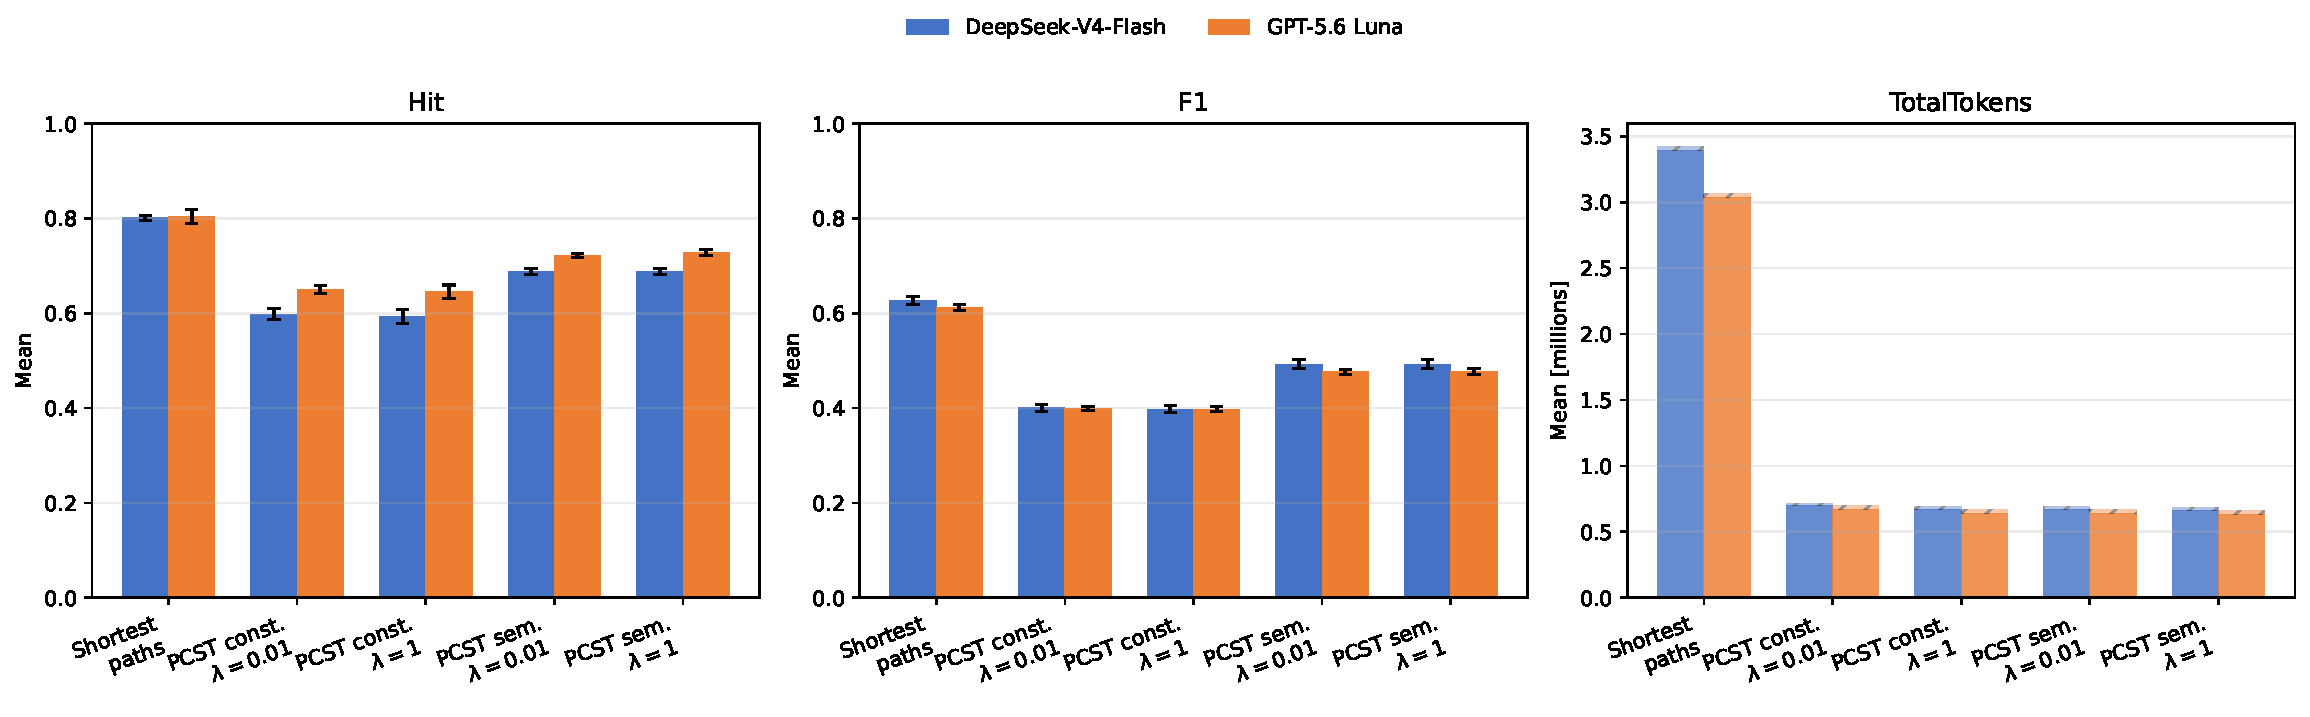
\includegraphics[width=\textwidth]{figures/end_to_end_llm_quality_tokens.pdf}
 \caption{Final Hit, micro F1, and total tokens for the two language models. Within each panel, configurations run from shortest paths to constant PCST ($\lambda=0.01,1$) and semantic PCST ($\lambda=0.01,1$). In the token panel, the main bar segment represents input tokens and the hatched segment output tokens. Values are means with standard deviations across three seed-associated runs; tokens are in millions.}
 \label{fig:quality-tokens}
\end{figure}

Constant-cost PCST causes the largest quality reduction. At $\lambda=1$, Hit falls to $0.594\pm0.014$ for DeepSeek and $0.645\pm0.015$ for GPT, decreases of approximately 20.8 and 15.9 percentage points from shortest paths. Both models reach F1 of approximately 0.398. Lowering $\lambda$ to 0.01 offers only small changes, although the low-cost construction retains every candidate. Candidate omission alone therefore cannot explain the observed quality gap.

Semantic PCST provides a better compact alternative. At $\lambda=1$, Hit is $0.689\pm0.006$ for DeepSeek and $0.728\pm0.006$ for GPT. F1 reaches $0.492\pm0.010$ and $0.477\pm0.006$, respectively. The two semantic endpoints perform similarly, while their improvement over constant costs is much larger. For the tested range, selecting the cost definition matters more for final quality than adjusting its scale between the two endpoints.

Shorter evidence reduces total tokens substantially. Shortest-path runs consume $3.42\pm0.77$ million tokens with DeepSeek and $3.07\pm0.66$ million with GPT; PCST configurations consume approximately 0.66--0.72 million. Relative reductions within each model are approximately 78--80\%. GPT with semantic PCST at $\lambda=1$ uses about 4.6 times fewer tokens than its shortest-path counterpart, while losing approximately 7.6 percentage points of Hit. The corresponding F1 drop, from 0.613 to 0.477, makes clear that this is a resource--quality trade-off rather than equivalent answering at lower cost. Appendix~\ref{app:final-results} reports all quality metrics and token totals.

\subsection{Context utilization and answer omissions}
\label{sec:context-results}

To distinguish answer-entity availability from answer completeness, we examine three related measures. FullContextCompleteAnswer is the fraction of evaluated questions for which the evidence contains every gold answer and the model returns all of them. FullContextLLMOmission uses the same overall denominator but counts fully covered questions where at least one gold answer is omitted. LLMOmissionGivenFullContext conditions its denominator on fully covered questions only (Appendix~\ref{app:metrics}). Returning an extra incorrect answer does not create an omission, although it can invalidate Exact Match.

Figure~\ref{fig:context-outcomes} shows that answer omissions persist even with high context coverage. For shortest paths, FullContextCompleteAnswer is $0.661\pm0.004$ with DeepSeek and $0.639\pm0.003$ with GPT. Their conditional omission rates are $0.211\pm0.002$ and $0.237\pm0.010$. Thus, even when every gold entity occurs in the evidence, at least one is missing from the generated answer in approximately one fifth to one quarter of questions.

\begin{figure}[t]
 \centering
 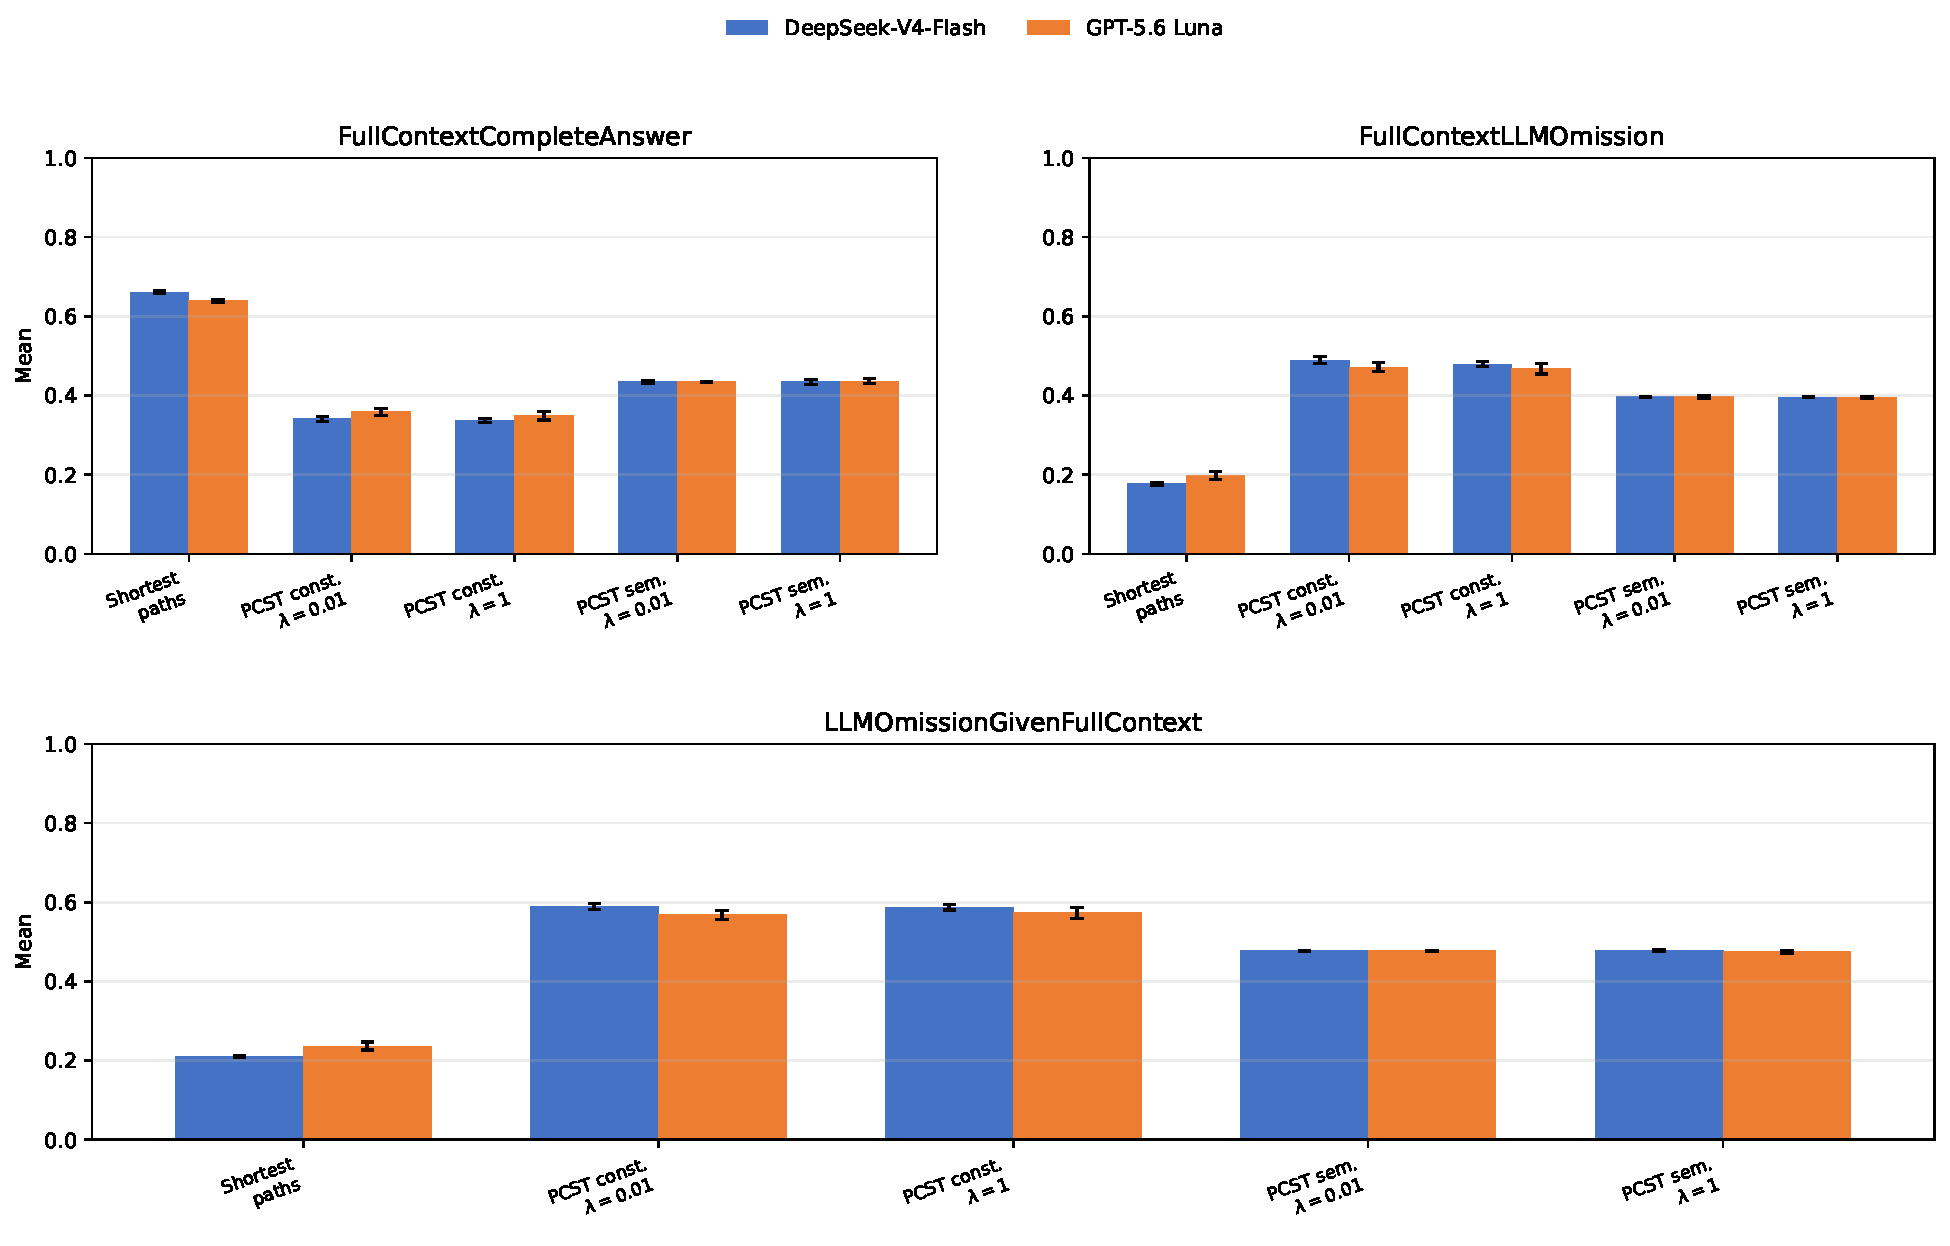
\includegraphics[width=0.88\textwidth]{figures/end_to_end_context_outcomes.pdf}
 \caption{Use of gold answers present in the evidence. The top panels show complete answers and omissions as fractions of all eligible questions; the bottom panel shows omissions conditional on full context coverage. Configuration order is the same as Figure~\ref{fig:quality-tokens}. Error bars indicate standard deviation across three runs. These measures test whether gold entities are returned, not whether the full set of predicted entities is exact.}
 \label{fig:context-outcomes}
\end{figure}

The discrepancy becomes larger after compression. Constant PCST at $\lambda=1$ has conditional omission rates of $0.587\pm0.007$ and $0.573\pm0.014$ for DeepSeek and GPT. Semantic PCST improves these to $0.477\pm0.003$ and $0.474\pm0.005$, respectively, but remains well above shortest paths. Meanwhile, full context coverage for semantic PCST is still $0.830\pm0.006$. The principal change is therefore not a large disappearance of answer entities from the context, but a reduced ability of the evidence-to-generation stage to return them all.

This result addresses RQ3 without assigning every omission solely to the language model. An entity can be visible without the evidence making its answer role clear. The removed triples may contain helpful alternative paths or relational qualifications; the present aggregate measurements do not identify which missing facts cause a particular failure. They do establish that compactness and entity presence are insufficient proxies for downstream evidence usefulness.

\section{Discussion}
\label{sec:discussion}

\subsection{What the architecture comparison establishes}

The observed ranking is consistent with the value of question-conditioned reasoning over paths. NBFNet and ReaRev achieve the strongest retrieval results, while a learned question-aware extension substantially improves the aggregation baseline. However, the experiment does not isolate question conditioning from model capacity, loss design, or representation choice. The evaluated configurations differ in hidden width, encoding, and normalization as well as in message passing. Their results are best interpreted as an assessment of practical implementations within a shared task and budget.

This distinction matters when relating the study to earlier methods. The results support the usefulness of an independently implemented GNN-guided workflow and expose substantial architectural sensitivity. They do not provide a direct performance comparison against published GNN-RAG numbers, whose full experimental protocol is not reproduced here. The replication-oriented contribution is the explicit reassessment of a recognizable pipeline under documented adaptations, followed by an examination of how those choices affect downstream behavior.

\subsection{Compact graphs are not necessarily sufficient evidence}

PCST and shortest-path union answer different structural questions. Shortest-path union retains all minimal alternatives linking candidates to the seed set; PCST favors a low-cost shared connection and can discard alternatives even when it keeps the candidates. The low-cost constant PCST result is especially informative: every candidate survives, yet final quality falls substantially. The benefit of the larger context consequently cannot be reduced to the inclusion of additional candidate entities.

Semantic costs recover part of the quality gap while preserving a similar triple budget. This is compatible with question--relation similarity selecting more useful connections, although it is not a direct semantic correctness test of individual edges. In particular, similarity does not guarantee that a set of triples jointly entails an answer. A relation that appears only weakly related to the question in isolation may still be essential to an intermediate step. The results motivate treating the sufficiency of relational evidence as a separate objective from node coverage and graph size.

Nor should the findings be generalized into a rule that longer contexts are always preferable. Only specific construction strategies are compared, and the larger context here contains the union of shortest paths. Its advantage could depend on which additional facts that strategy preserves. The supported conclusion is that this particular compression trades away useful answering information or accessibility despite high entity retention.

\subsection{Why intermediate evaluation matters}

The workflow is not a strictly decreasing sequence of answer sets. Evidence construction may reveal correct intermediate entities absent from the candidate list, explaining why context gold coverage can be slightly higher than retrieval coverage. A final model may also fail to return entities already visible in its context. Measuring only candidate hits or only final accuracy would hide both effects.

The conditional omission metric makes one downstream limitation explicit without comparing incompatible averages. Retrieval and context coverage are macro averages over questions; final recall pools answer counts across questions. Their numerical difference is therefore not a valid estimate of a stage-specific loss probability. Conditioning omissions on full context coverage instead identifies questions for which answer-entity absence is insufficient to explain the failure. It still leaves open whether the supplied relations are inadequate, the generator misinterprets them, normalization misses an equivalent name, or a generation fails.

Within this scope, the evidence-to-answer transition is a substantial bottleneck. Both language models show high omissions after compression, and neither turns entity coverage into complete answers reliably. The models also respond differently to evidence strategies: GPT achieves higher Hit on compact contexts, whereas DeepSeek maintains higher precision and F1 in the semantic conditions. A single metric would obscure these differences. Joint reporting of answer completeness, selectivity, and resource use provides a more useful basis for choosing a configuration.

\section{Limitations}
\label{sec:limitations}

The study uses one dataset and supplied local graphs with given seed entities. Excluding graphs without all labeled answers conditions the findings on upstream graph completeness and removes entity-linking failures from consideration. The combined validation/test evaluation and downstream selection of NBFNet on that evaluation pool mean that these numbers are comparative results under this protocol, not an independently held-out estimate for a selected system or a directly comparable WebQSP leaderboard result.

Only one configuration per architecture and three random seeds are evaluated. Architectures differ in question access, embeddings, capacity, and objective, so the comparison does not attribute improvements to individual components or establish statistical significance. Some methods are adapted from tasks other than KGQA. Downstream experiments use NBFNet only, leaving interactions between other retrievers and evidence builders unmeasured.

The generation comparison covers two recorded API model configurations with a common answer-only prompt. The three repetitions inherit different retriever seeds and their evidence; they are not three isolated measurements of generator randomness on identical contexts. Entity-name normalization and label completeness also limit exact set-based scoring. Token counts are useful within-model resource indicators but do not establish comparable financial cost or latency across providers. Finally, context-coverage metrics measure entity occurrence, not logical sufficiency, and the study does not identify the precise cause of each omission.

\section{Conclusion}
\label{sec:conclusion}

This study reassesses GNN-guided knowledge graph question answering through its retrieval, evidence-construction, and generation stages. Among the six evaluated retrievers, NBFNet achieves the strongest mean ranking and coverage results with low variation across seeds. The comparison also shows that an extended question-aware GraphSAGE implementation can improve substantially over the weighted aggregation baseline, while relation-specific modeling alone is insufficient to ensure stronger retrieval in the tested configurations.

Rooted PCST compresses evidence by approximately 85\% and reduces token use by approximately 78--80\%, largely preserving answer-entity coverage. This compression nevertheless lowers final answer quality. Semantic costs provide the stronger compact alternative, but shortest-path union remains the best-performing evidence strategy for both language models. Conditional omissions demonstrate that many correct entities present in the context are still not returned, especially after compression.

The resulting design lesson is to assess evidence through what it enables the generator to answer, as well as through what it contains. Future work can investigate hybrid evidence selection that preserves informative paths, objectives connected to answer completeness, and joint optimization of retrieval and evidence construction. Such extensions should be evaluated across additional datasets and configurations. Effective GNN-guided answering requires candidate relevance, sufficient relational evidence, and successful context use to be considered together.

\bibliography{references}
\bibliographystyle{tmlr}

\clearpage
\appendix
\section{Architecture and training details}
\label{app:architectures}

Table~\ref{tab:architecture-settings} records the architecture settings in the current experiment manifest. Widths and internal computation differ; a shared number of training epochs does not imply equal parameter counts or compute. The baseline named GraphSAGE is the weighted implementation described in Section~\ref{sec:architectures}, and \method{} denotes the combined extension used in the study.

\begin{table}[h]
 \centering
 \caption{Fixed retrieval configurations. ``3/3/3'' denotes ReaRev's instructions, reasoning steps, and adaptive iterations, respectively. Dropout 0.1 is explicitly configured for the first five models; NBFNet uses its fixed path-propagation implementation. Settings are reproduced from the experiment manifest.}
 \label{tab:architecture-settings}
 \begingroup
\small
\begin{tabularx}{\textwidth}{@{}lccX@{}}
\toprule
Architecture & Width & Depth & Main configured characteristics \\
\midrule
GraphSAGE & 256 & 3 & Fixed cosine edge weights; MLP node classifier. \\
\method{} & 256 & 3 & Learned edge MLP (width 256), reverse edges, residual normalization, question-aware classifier. \\
R-GCN & 256 & 3 & 30 relation bases; categorical forward/reverse relations. \\
HGT & 128 & $3^{\dagger}$ & 8 attention heads; one entity node type; relation-dependent attention. \\
ReaRev & 50 & 3/3/3 & Frozen MiniLM; token instructions; adaptive revision. \\
NBFNet & 32 & 3 & Question-conditioned boundary states; DistMult messages; PNA aggregation. \\
\bottomrule
\end{tabularx}
\endgroup

 \par\smallskip
 {\footnotesize\raggedright $\dagger$ The current manifest uses three HGT layers. Its seed-1337 entry was corrected from two to three after the recorded run date; the saved summary does not establish that run's depth. Historical configuration verification is pending, so the HGT variability must not yet be interpreted as purely seed-induced.\par}
\end{table}

\paragraph{Aggregation variants.}
For an incoming triple $(u,r,v)$, the GraphSAGE implementation sums weighted transformed source states and concatenates this sum with the current target state before a learned update. The baseline weight is cosine question--relation similarity. \method{} uses Equation~\ref{eq:gate} and the residual-normalized update $\mathbf h_v^{(\ell+1)}=\operatorname{ReLU}(\operatorname{LayerNorm}(\mathbf h_v^{(\ell)}+\operatorname{Dropout}(\mathbf u_v^{(\ell)})))$, where $\mathbf u_v^{(\ell)}$ is the message-passing update. R-GCN uses $W_r^{(\ell)}=\sum_{b=1}^{30}a_{rb}^{(\ell)}V_b^{(\ell)}$ and relation-wise neighbor normalization. Its forward and reverse relations have separate identifiers. HGT retains relation-specific attention and message transformations with eight heads, shared node-type projections, a learned residual gate, and normalization.

\paragraph{Task-oriented models.}
ReaRev uses the frozen encoder \texttt{sentence-transformers/all-MiniLM-L6-v2}, revision \texttt{1110a243fdf4706b3f48f1d95db1a4f5529b4d41}, with maximum question and relation lengths of 64 and 16 tokens. Token-level attention produces three instructions. Initial entity states derive from incident relation information, and reasoning begins from a seed distribution. Instructions are revised after each reasoning iteration. NBFNet supplies the full projected question vector to each seed, uses separate original and reverse relation operators, and reinjects the initial boundary condition at each layer. PNA combines mean, maximum, minimum, and standard deviation statistics with degree scaling \citep{corso2020pna}. Final node states are concatenated with the question representation for scoring.

\paragraph{Training objective.}
All models except ReaRev use independent binary answer labels and class-balanced binary cross-entropy. For a graph with $n_+$ positive and $n_-$ negative nodes, the positive term receives weight $n_-/n_+$ when $n_+>0$. ReaRev instead minimizes KL divergence to a distribution uniform over the gold answer nodes. Independent outputs are passed through sigmoid, whereas ReaRev yields a softmax distribution. The common candidate-selection rule is applied after these normalizations. The model comparison therefore includes differences in objective and calibration, as well as architecture.

\section{Metric definitions and evaluation protocol}
\label{app:metrics}

Let $Q$ be the set of evaluated questions with nonempty normalized gold sets and $N=|Q|=1746$. Let $C_q^{(k)}$ be the top $k$ retrieved candidates, $C_q$ the final candidate set, $U_q$ the source and target entities actually appearing in emitted evidence triples, and $P_q$ the normalized prediction set. The indicator function $\ind[\cdot]$ is one when its argument holds. Reported standard deviations are computed over the three run-level values, using denominator $3-1$.

\paragraph{Retrieval.}
Hits@k measures whether at least one gold answer appears in the first $k$ candidates:
\begin{equation}
 \operatorname{Hits@}k=\frac1N\sum_{q\in Q}\ind[A_q\cap C_q^{(k)}\ne\varnothing],
 \quad
 \operatorname{nDCG@}k=\frac1N\sum_{q\in Q}
 \frac{\sum_{i=1}^{k}\mathrm{rel}_{qi}/\log_2(i+1)}
 {\sum_{i=1}^{\min(|A_q|,k)}1/\log_2(i+1)}.
\end{equation}
Relevance is binary, and nonexistent candidate positions contribute zero. nDCG rewards earlier relevant results and normalizes by an ideal list \citep{jarvelin2002cumulated}. The coverage metrics in Table~\ref{tab:retrieval} are
\begin{equation}
 \operatorname{RGC}=\frac1N\sum_{q\in Q}\frac{|A_q\cap C_q|}{|A_q|},
 \qquad
 \operatorname{RFGC}=\frac1N\sum_{q\in Q}\ind[A_q\subseteq C_q].
\end{equation}
Both are macro averages: each question has equal weight regardless of its answer-set size.

\paragraph{Evidence.}
AverageTriples is $N^{-1}\sum_q|H_q|$ and AverageDistinctNodes is $N^{-1}\sum_q|U_q|$. Let $D_q$ be the retrieved candidates retained according to the construction output. ContextCandidateCoverage is the macro average of $|D_q|/|C_q|$, with zero for an empty candidate list. CandidateReduction instead pools counts: $100\sum_q(|C_q|-|D_q|)/\sum_q|C_q|$. These two aggregates need not be exact complements. ContextGoldCoverage (CGC) and ContextFullGoldCoverage (CFGC) replace $C_q$ by $U_q$ in the RGC and RFGC formulas. Candidate retention and evidence visibility are distinct: a seed-only, zero-edge structure does not expose an entity in a serialized triple.

\paragraph{Final answer quality.}
Hit is $N^{-1}\sum_q\ind[A_q\cap P_q\ne\varnothing]$, and Exact Match (EM) is $N^{-1}\sum_q\ind[A_q=P_q]$. For micro metrics, $\mathrm{TP}=\sum_q|A_q\cap P_q|$, $\mathrm{FP}=\sum_q|P_q\setminus A_q|$, and $\mathrm{FN}=\sum_q|A_q\setminus P_q|$. Precision is $\mathrm{TP}/(\mathrm{TP}+\mathrm{FP})$, recall is $\mathrm{TP}/(\mathrm{TP}+\mathrm{FN})$, and F1 is their harmonic mean. Zero denominators yield zero. Failed generations use an empty prediction set and are forced to fail EM. These pooled metrics weight individual answers rather than questions.

\paragraph{Context utilization.}
Define $F_q=\ind[A_q\subseteq U_q]$ and $O_q=\ind[A_q\nsubseteq P_q]$. The two full-context outcomes and the conditional omission rate are
\begin{align}
 \operatorname{FullContextCompleteAnswer}&=\frac1N\sum_q F_q(1-O_q),\\
 \operatorname{FullContextLLMOmission}&=\frac1N\sum_q F_qO_q,\\
 \operatorname{LLMOmissionGivenFullContext}&=\frac{\sum_q F_qO_q}{\sum_q F_q}.
 \label{eq:conditional-omission}
\end{align}
The last metric is undefined if no question has full context coverage; that case does not occur in the displayed results. The first two rates sum to CFGC for each run, not to one. Completeness allows extra predicted entities, while Exact Match does not. Conditional rates are computed within each run before averaging; dividing already averaged rates can give a different value.

\paragraph{Normalization and accounting.}
Answer strings are lowercased and trimmed; punctuation and English articles are removed, whitespace is collapsed, and duplicate normalized answers are removed. Comparisons use these normalized names rather than a learned semantic-equivalence judge. Per-stage records are joined by instance identifier. TotalTokens sums recorded input and output usage for a run, including instructions and question tokens as well as evidence. Resource comparisons are made primarily within a language model because tokenizers differ.

\section{Complete evidence-construction results}
\label{app:evidence-results}

Table~\ref{tab:evidence-full} reports all nine evidence settings. The three NBFNet seeds are reused throughout. PCST operates on a multigraph of original facts, with no synthetic inverse facts in the output. The implementation calls \texttt{pcst\_fast} with a specified root, one cluster, and \texttt{gw} pruning. For multiple seeds, each seed receives an additional prize greater than the sum of candidate prizes and structural edge costs, and is connected to a temporary root at zero cost. Removing that root can leave multiple seed-anchored branches. The quoted candidate prizes and reported collected prize exclude these enforcement additions.

\begin{table}[h]
 \centering
 \caption{Evidence results, mean $\pm$ standard deviation across three NBFNet seeds. CCC: macro candidate coverage; Red.: pooled candidate reduction in percent; CGC: context gold coverage; CFGC: full context gold coverage. Constant and semantic rows differ only in their edge-cost definition and scale.}
 \label{tab:evidence-full}
 \begingroup
\footnotesize
\setlength{\tabcolsep}{3pt}
\begin{tabular}{@{}lccccccc@{}}
\toprule
Strategy & $\lambda$ & Triples & Nodes & CCC & Red. (\%) & CGC & CFGC \\
\midrule
Shortest paths & -- & $94.47\pm22.58$ & $32.12\pm6.60$ & $1.000\pm0.000$ & $0.00\pm0.00$ & $0.888\pm0.006$ & $0.838\pm0.007$ \\
\midrule
PCST constant & 0.01 & $14.45\pm0.26$ & $15.46\pm0.26$ & $1.000\pm0.000$ & $0.00\pm0.00$ & $0.881\pm0.004$ & $0.831\pm0.005$ \\
 & 0.25 & $14.45\pm0.26$ & $15.46\pm0.26$ & $1.000\pm0.000$ & $0.00\pm0.00$ & $0.881\pm0.004$ & $0.831\pm0.005$ \\
 & 0.5 & $14.30\pm0.25$ & $15.31\pm0.25$ & $0.994\pm0.003$ & $0.61\pm0.30$ & $0.881\pm0.004$ & $0.830\pm0.006$ \\
 & 1 & $13.57\pm0.26$ & $14.58\pm0.26$ & $0.949\pm0.003$ & $5.02\pm0.33$ & $0.875\pm0.003$ & $0.816\pm0.005$ \\
\midrule
PCST semantic & 0.01 & $13.70\pm0.28$ & $14.71\pm0.28$ & $1.000\pm0.000$ & $0.00\pm0.00$ & $0.881\pm0.004$ & $0.831\pm0.006$ \\
 & 0.25 & $13.70\pm0.28$ & $14.71\pm0.28$ & $1.000\pm0.000$ & $0.00\pm0.00$ & $0.881\pm0.004$ & $0.831\pm0.006$ \\
 & 0.5 & $13.70\pm0.28$ & $14.71\pm0.28$ & $1.000\pm0.000$ & $0.00\pm0.00$ & $0.881\pm0.004$ & $0.831\pm0.006$ \\
 & 1 & $13.50\pm0.24$ & $14.51\pm0.24$ & $0.991\pm0.004$ & $0.82\pm0.38$ & $0.881\pm0.004$ & $0.830\pm0.006$ \\
\bottomrule
\end{tabular}
\endgroup

\end{table}

The table highlights why candidate survival alone cannot determine context usefulness. Both costs at $\lambda=0.01$ retain all retrieved candidates, and their CGC values round to the same number, while downstream answer quality differs substantially. The measured difference is associated with the selected connecting structure, not with a wholesale reduction in candidate availability. Similar rounded aggregates are not evidence that the individual subgraphs are identical.

\section{Complete final results and reproducibility details}
\label{app:final-results}

Table~\ref{tab:final-full} gives all ten model--evidence combinations. Each row summarizes three runs associated with the same three NBFNet retriever seeds. Table~\ref{tab:omission-full} provides the exact conditional rates used in Section~\ref{sec:context-results}, including the low-cost endpoints. No additional training or inference runs were introduced to prepare these tables.

\begin{table}[h]
 \centering
 \caption{Complete final-answer results. P and R are micro precision and recall; EM is Exact Match; tokens are total input plus output tokens in millions per run. SP denotes shortest-path union, C constant PCST, and S semantic PCST. All entries are mean $\pm$ standard deviation across three runs.}
 \label{tab:final-full}
 \begingroup
\footnotesize
\setlength{\tabcolsep}{4pt}
\begin{tabular}{@{}lcccccc@{}}
\toprule
Evidence & Hit & P & R & F1 & EM & Tokens (M) \\
\midrule
\multicolumn{7}{@{}l}{\textbf{DeepSeek-V4-Flash}} \\
SP & $0.802\pm0.005$ & $0.860\pm0.009$ & $0.493\pm0.007$ & $0.627\pm0.008$ & $0.580\pm0.003$ & $3.42\pm0.77$ \\
C, $\lambda=0.01$ & $0.598\pm0.012$ & $0.881\pm0.006$ & $0.259\pm0.005$ & $0.400\pm0.007$ & $0.322\pm0.002$ & $0.72\pm0.01$ \\
C, $\lambda=1$ & $0.594\pm0.014$ & $0.884\pm0.007$ & $0.257\pm0.006$ & $0.398\pm0.008$ & $0.320\pm0.002$ & $0.69\pm0.01$ \\
S, $\lambda=0.01$ & $0.688\pm0.007$ & $0.885\pm0.008$ & $0.342\pm0.008$ & $0.493\pm0.010$ & $0.410\pm0.003$ & $0.69\pm0.01$ \\
S, $\lambda=1$ & $0.689\pm0.006$ & $0.886\pm0.008$ & $0.341\pm0.008$ & $0.492\pm0.010$ & $0.411\pm0.004$ & $0.69\pm0.01$ \\
\midrule
\multicolumn{7}{@{}l}{\textbf{GPT-5.6 Luna}} \\
SP & $0.804\pm0.015$ & $0.846\pm0.007$ & $0.481\pm0.006$ & $0.613\pm0.006$ & $0.571\pm0.006$ & $3.07\pm0.66$ \\
C, $\lambda=0.01$ & $0.651\pm0.009$ & $0.847\pm0.001$ & $0.261\pm0.004$ & $0.399\pm0.005$ & $0.341\pm0.006$ & $0.70\pm0.01$ \\
C, $\lambda=1$ & $0.645\pm0.015$ & $0.849\pm0.006$ & $0.260\pm0.004$ & $0.398\pm0.006$ & $0.331\pm0.009$ & $0.67\pm0.01$ \\
S, $\lambda=0.01$ & $0.723\pm0.004$ & $0.850\pm0.008$ & $0.331\pm0.004$ & $0.476\pm0.005$ & $0.414\pm0.003$ & $0.67\pm0.01$ \\
S, $\lambda=1$ & $0.728\pm0.006$ & $0.854\pm0.007$ & $0.331\pm0.006$ & $0.477\pm0.006$ & $0.414\pm0.005$ & $0.66\pm0.01$ \\
\bottomrule
\end{tabular}
\endgroup

\end{table}

\begin{table}[h]
 \centering
 \caption{LLMOmissionGivenFullContext for every evaluated evidence setting. Lower is better. Conditioning is on full gold-entity coverage in each run's evidence, not on a shared fixed subset across all construction strategies.}
 \label{tab:omission-full}
 \begingroup
\small
\begin{tabular}{@{}lcc@{}}
\toprule
Evidence & DeepSeek-V4-Flash & GPT-5.6 Luna \\
\midrule
Shortest paths & $0.211\pm0.002$ & $0.237\pm0.010$ \\
PCST constant, $\lambda=0.01$ & $0.589\pm0.008$ & $0.568\pm0.012$ \\
PCST constant, $\lambda=1$ & $0.587\pm0.007$ & $0.573\pm0.014$ \\
PCST semantic, $\lambda=0.01$ & $0.477\pm0.001$ & $0.477\pm0.002$ \\
PCST semantic, $\lambda=1$ & $0.477\pm0.003$ & $0.474\pm0.005$ \\
\bottomrule
\end{tabular}
\endgroup

\end{table}

\paragraph{Generation protocol.}
The configured API model identifiers are \texttt{deepseek-v4-flash} and \texttt{gpt-5.6-luna}; these names identify the recorded runs. The generation service requests temperature zero. It supplies the question, deduplicated directed triples, and a common answer-only instruction requiring JSON of the form \texttt{\{"answers": ["complete entity name"]\}}. Entity names containing commas must remain a single item. Unsupported questions should return an empty array, and explanations are disabled. The system instruction reads:
\begin{quote}\small
You answer questions using only the provided reasoning paths. Return only valid JSON with the key answers. The answers value must be a JSON array of complete entity names. Do not generate an explanation. If the paths do not support an answer, return an empty answers array.
\end{quote}

\paragraph{Recorded artifacts.}
The implementation separates training, retriever evaluation, evidence construction, and inference outputs. Experiment manifests pin the three seeds and map the six retrievers, nine evidence conditions, and ten final conditions to persisted runs. The analysis comprises 18 retrieval runs, 27 evidence runs, and 30 final-generation runs. Result exports retain per-run values, aggregated summaries, and source-run provenance, allowing tables to be regenerated from existing measurements. Numeric experiment identifiers in the implementation are zero-based; the scientific comparisons here are organized by stage rather than identifier.

\paragraph{Scope of reproducibility.}
Training uses PyTorch and the settings in Section~\ref{sec:setup}; graph preparation and name mapping are part of the recorded pipeline. Exact reproduction also depends on the original prepared dataset, encoder artifacts, and API model availability. The comparison is between fixed implementations, with their different input encoders and objectives, and does not establish equal computational budgets. Public repository and tracking links are omitted from this anonymous draft. A review-ready anonymous artifact link must be supplied separately before submission; no anonymous archive is claimed to have been deposited here.


\end{document}
